% Options for packages loaded elsewhere
% Options for packages loaded elsewhere
\PassOptionsToPackage{unicode}{hyperref}
\PassOptionsToPackage{hyphens}{url}
\PassOptionsToPackage{dvipsnames,svgnames,x11names}{xcolor}
%
\documentclass[
  12pt,
  letterpaper,
  DIV=11,
  numbers=noendperiod]{scrartcl}
\usepackage{xcolor}
\usepackage{amsmath,amssymb}
\setcounter{secnumdepth}{5}
\usepackage{iftex}
\ifPDFTeX
  \usepackage[T1]{fontenc}
  \usepackage[utf8]{inputenc}
  \usepackage{textcomp} % provide euro and other symbols
\else % if luatex or xetex
  \usepackage{unicode-math} % this also loads fontspec
  \defaultfontfeatures{Scale=MatchLowercase}
  \defaultfontfeatures[\rmfamily]{Ligatures=TeX,Scale=1}
\fi
\usepackage{lmodern}
\ifPDFTeX\else
  % xetex/luatex font selection
  \setmainfont[]{Times New Roman}
\fi
% Use upquote if available, for straight quotes in verbatim environments
\IfFileExists{upquote.sty}{\usepackage{upquote}}{}
\IfFileExists{microtype.sty}{% use microtype if available
  \usepackage[]{microtype}
  \UseMicrotypeSet[protrusion]{basicmath} % disable protrusion for tt fonts
}{}
\makeatletter
\@ifundefined{KOMAClassName}{% if non-KOMA class
  \IfFileExists{parskip.sty}{%
    \usepackage{parskip}
  }{% else
    \setlength{\parindent}{0pt}
    \setlength{\parskip}{6pt plus 2pt minus 1pt}}
}{% if KOMA class
  \KOMAoptions{parskip=half}}
\makeatother
% Make \paragraph and \subparagraph free-standing
\makeatletter
\ifx\paragraph\undefined\else
  \let\oldparagraph\paragraph
  \renewcommand{\paragraph}{
    \@ifstar
      \xxxParagraphStar
      \xxxParagraphNoStar
  }
  \newcommand{\xxxParagraphStar}[1]{\oldparagraph*{#1}\mbox{}}
  \newcommand{\xxxParagraphNoStar}[1]{\oldparagraph{#1}\mbox{}}
\fi
\ifx\subparagraph\undefined\else
  \let\oldsubparagraph\subparagraph
  \renewcommand{\subparagraph}{
    \@ifstar
      \xxxSubParagraphStar
      \xxxSubParagraphNoStar
  }
  \newcommand{\xxxSubParagraphStar}[1]{\oldsubparagraph*{#1}\mbox{}}
  \newcommand{\xxxSubParagraphNoStar}[1]{\oldsubparagraph{#1}\mbox{}}
\fi
\makeatother

\usepackage{color}
\usepackage{fancyvrb}
\newcommand{\VerbBar}{|}
\newcommand{\VERB}{\Verb[commandchars=\\\{\}]}
\DefineVerbatimEnvironment{Highlighting}{Verbatim}{commandchars=\\\{\}}
% Add ',fontsize=\small' for more characters per line
\usepackage{framed}
\definecolor{shadecolor}{RGB}{241,243,245}
\newenvironment{Shaded}{\begin{snugshade}}{\end{snugshade}}
\newcommand{\AlertTok}[1]{\textcolor[rgb]{0.68,0.00,0.00}{#1}}
\newcommand{\AnnotationTok}[1]{\textcolor[rgb]{0.37,0.37,0.37}{#1}}
\newcommand{\AttributeTok}[1]{\textcolor[rgb]{0.40,0.45,0.13}{#1}}
\newcommand{\BaseNTok}[1]{\textcolor[rgb]{0.68,0.00,0.00}{#1}}
\newcommand{\BuiltInTok}[1]{\textcolor[rgb]{0.00,0.23,0.31}{#1}}
\newcommand{\CharTok}[1]{\textcolor[rgb]{0.13,0.47,0.30}{#1}}
\newcommand{\CommentTok}[1]{\textcolor[rgb]{0.37,0.37,0.37}{#1}}
\newcommand{\CommentVarTok}[1]{\textcolor[rgb]{0.37,0.37,0.37}{\textit{#1}}}
\newcommand{\ConstantTok}[1]{\textcolor[rgb]{0.56,0.35,0.01}{#1}}
\newcommand{\ControlFlowTok}[1]{\textcolor[rgb]{0.00,0.23,0.31}{\textbf{#1}}}
\newcommand{\DataTypeTok}[1]{\textcolor[rgb]{0.68,0.00,0.00}{#1}}
\newcommand{\DecValTok}[1]{\textcolor[rgb]{0.68,0.00,0.00}{#1}}
\newcommand{\DocumentationTok}[1]{\textcolor[rgb]{0.37,0.37,0.37}{\textit{#1}}}
\newcommand{\ErrorTok}[1]{\textcolor[rgb]{0.68,0.00,0.00}{#1}}
\newcommand{\ExtensionTok}[1]{\textcolor[rgb]{0.00,0.23,0.31}{#1}}
\newcommand{\FloatTok}[1]{\textcolor[rgb]{0.68,0.00,0.00}{#1}}
\newcommand{\FunctionTok}[1]{\textcolor[rgb]{0.28,0.35,0.67}{#1}}
\newcommand{\ImportTok}[1]{\textcolor[rgb]{0.00,0.46,0.62}{#1}}
\newcommand{\InformationTok}[1]{\textcolor[rgb]{0.37,0.37,0.37}{#1}}
\newcommand{\KeywordTok}[1]{\textcolor[rgb]{0.00,0.23,0.31}{\textbf{#1}}}
\newcommand{\NormalTok}[1]{\textcolor[rgb]{0.00,0.23,0.31}{#1}}
\newcommand{\OperatorTok}[1]{\textcolor[rgb]{0.37,0.37,0.37}{#1}}
\newcommand{\OtherTok}[1]{\textcolor[rgb]{0.00,0.23,0.31}{#1}}
\newcommand{\PreprocessorTok}[1]{\textcolor[rgb]{0.68,0.00,0.00}{#1}}
\newcommand{\RegionMarkerTok}[1]{\textcolor[rgb]{0.00,0.23,0.31}{#1}}
\newcommand{\SpecialCharTok}[1]{\textcolor[rgb]{0.37,0.37,0.37}{#1}}
\newcommand{\SpecialStringTok}[1]{\textcolor[rgb]{0.13,0.47,0.30}{#1}}
\newcommand{\StringTok}[1]{\textcolor[rgb]{0.13,0.47,0.30}{#1}}
\newcommand{\VariableTok}[1]{\textcolor[rgb]{0.07,0.07,0.07}{#1}}
\newcommand{\VerbatimStringTok}[1]{\textcolor[rgb]{0.13,0.47,0.30}{#1}}
\newcommand{\WarningTok}[1]{\textcolor[rgb]{0.37,0.37,0.37}{\textit{#1}}}

\usepackage{longtable,booktabs,array}
\usepackage{calc} % for calculating minipage widths
% Correct order of tables after \paragraph or \subparagraph
\usepackage{etoolbox}
\makeatletter
\patchcmd\longtable{\par}{\if@noskipsec\mbox{}\fi\par}{}{}
\makeatother
% Allow footnotes in longtable head/foot
\IfFileExists{footnotehyper.sty}{\usepackage{footnotehyper}}{\usepackage{footnote}}
\makesavenoteenv{longtable}
\usepackage{graphicx}
\makeatletter
\newsavebox\pandoc@box
\newcommand*\pandocbounded[1]{% scales image to fit in text height/width
  \sbox\pandoc@box{#1}%
  \Gscale@div\@tempa{\textheight}{\dimexpr\ht\pandoc@box+\dp\pandoc@box\relax}%
  \Gscale@div\@tempb{\linewidth}{\wd\pandoc@box}%
  \ifdim\@tempb\p@<\@tempa\p@\let\@tempa\@tempb\fi% select the smaller of both
  \ifdim\@tempa\p@<\p@\scalebox{\@tempa}{\usebox\pandoc@box}%
  \else\usebox{\pandoc@box}%
  \fi%
}
% Set default figure placement to htbp
\def\fps@figure{htbp}
\makeatother


% definitions for citeproc citations
\NewDocumentCommand\citeproctext{}{}
\NewDocumentCommand\citeproc{mm}{%
  \begingroup\def\citeproctext{#2}\cite{#1}\endgroup}
\makeatletter
 % allow citations to break across lines
 \let\@cite@ofmt\@firstofone
 % avoid brackets around text for \cite:
 \def\@biblabel#1{}
 \def\@cite#1#2{{#1\if@tempswa , #2\fi}}
\makeatother
\newlength{\cslhangindent}
\setlength{\cslhangindent}{1.5em}
\newlength{\csllabelwidth}
\setlength{\csllabelwidth}{3em}
\newenvironment{CSLReferences}[2] % #1 hanging-indent, #2 entry-spacing
 {\begin{list}{}{%
  \setlength{\itemindent}{0pt}
  \setlength{\leftmargin}{0pt}
  \setlength{\parsep}{0pt}
  % turn on hanging indent if param 1 is 1
  \ifodd #1
   \setlength{\leftmargin}{\cslhangindent}
   \setlength{\itemindent}{-1\cslhangindent}
  \fi
  % set entry spacing
  \setlength{\itemsep}{#2\baselineskip}}}
 {\end{list}}
\usepackage{calc}
\newcommand{\CSLBlock}[1]{\hfill\break\parbox[t]{\linewidth}{\strut\ignorespaces#1\strut}}
\newcommand{\CSLLeftMargin}[1]{\parbox[t]{\csllabelwidth}{\strut#1\strut}}
\newcommand{\CSLRightInline}[1]{\parbox[t]{\linewidth - \csllabelwidth}{\strut#1\strut}}
\newcommand{\CSLIndent}[1]{\hspace{\cslhangindent}#1}



\setlength{\emergencystretch}{3em} % prevent overfull lines

\providecommand{\tightlist}{%
  \setlength{\itemsep}{0pt}\setlength{\parskip}{0pt}}



 


\usepackage{tcolorbox}
\usepackage{amssymb}
\usepackage{yfonts}
\usepackage{bm}


\newtcolorbox{greybox}{
  colback=white,
  colframe=blue,
  coltext=black,
  boxsep=5pt,
  arc=4pt}
  
\newcommand{\sectionbreak}{\clearpage}

 
\newcommand{\ds}[4]{\sum_{{#1}=1}^{#3}\sum_{{#2}=1}^{#4}}
\newcommand{\us}[3]{\mathop{\sum\sum}_{1\leq{#2}<{#1}\leq{#3}}}

\newcommand{\ol}[1]{\overline{#1}}
\newcommand{\ul}[1]{\underline{#1}}

\newcommand{\amin}[1]{\mathop{\text{argmin}}_{#1}}
\newcommand{\amax}[1]{\mathop{\text{argmax}}_{#1}}

\newcommand{\ci}{\perp\!\!\!\perp}

\newcommand{\mc}[1]{\mathcal{#1}}
\newcommand{\mb}[1]{\mathbb{#1}}
\newcommand{\mf}[1]{\mathfrak{#1}}

\newcommand{\eps}{\epsilon}
\newcommand{\lbd}{\lambda}
\newcommand{\alp}{\alpha}
\newcommand{\df}{=:}
\newcommand{\am}[1]{\mathop{\text{argmin}}_{#1}}
\newcommand{\ls}[2]{\mathop{\sum\sum}_{#1}^{#2}}
\newcommand{\ijs}{\mathop{\sum\sum}_{1\leq i<j\leq n}}
\newcommand{\jis}{\mathop{\sum\sum}_{1\leq j<i\leq n}}
\newcommand{\sij}{\sum_{i=1}^n\sum_{j=1}^n}
	
\KOMAoption{captions}{tableheading}
\makeatletter
\@ifpackageloaded{caption}{}{\usepackage{caption}}
\AtBeginDocument{%
\ifdefined\contentsname
  \renewcommand*\contentsname{Table of contents}
\else
  \newcommand\contentsname{Table of contents}
\fi
\ifdefined\listfigurename
  \renewcommand*\listfigurename{List of Figures}
\else
  \newcommand\listfigurename{List of Figures}
\fi
\ifdefined\listtablename
  \renewcommand*\listtablename{List of Tables}
\else
  \newcommand\listtablename{List of Tables}
\fi
\ifdefined\figurename
  \renewcommand*\figurename{Figure}
\else
  \newcommand\figurename{Figure}
\fi
\ifdefined\tablename
  \renewcommand*\tablename{Table}
\else
  \newcommand\tablename{Table}
\fi
}
\@ifpackageloaded{float}{}{\usepackage{float}}
\floatstyle{ruled}
\@ifundefined{c@chapter}{\newfloat{codelisting}{h}{lop}}{\newfloat{codelisting}{h}{lop}[chapter]}
\floatname{codelisting}{Listing}
\newcommand*\listoflistings{\listof{codelisting}{List of Listings}}
\makeatother
\makeatletter
\makeatother
\makeatletter
\@ifpackageloaded{caption}{}{\usepackage{caption}}
\@ifpackageloaded{subcaption}{}{\usepackage{subcaption}}
\makeatother
\usepackage{bookmark}
\IfFileExists{xurl.sty}{\usepackage{xurl}}{} % add URL line breaks if available
\urlstyle{same}
\hypersetup{
  pdftitle={Variations on a Theme by Eckart and Young},
  pdfauthor={Jan de Leeuw; Jan Graffelman},
  colorlinks=true,
  linkcolor={blue},
  filecolor={Maroon},
  citecolor={Blue},
  urlcolor={Blue},
  pdfcreator={LaTeX via pandoc}}


\title{Variations on a Theme by Eckart and Young}
\author{Jan de Leeuw \and Jan Graffelman}
\date{September 27, 2025}
\begin{document}
\maketitle
\begin{abstract}
TBD
\end{abstract}

\renewcommand*\contentsname{Table of contents}
{
\hypersetup{linkcolor=}
\setcounter{tocdepth}{3}
\tableofcontents
}

\sectionbreak

\textbf{Note:} This is a working manuscript which will be
expanded/updated frequently. All suggestions for improvement are
welcome. All Rmd, tex, html, pdf, R, and C files are in the public
domain. Attribution will be appreciated, but is not required. The files
can be found at \url{https://github.com/deleeuw/glspca}

\sectionbreak

\section{Introduction}\label{introduction}

\(X\) is a ``tall'' matrix of rank \(r\) with \(n\) rows and \(m\)
columns, \(r\leq m\leq n\). We want to approximate \(A\) in the
least-squarese sense by the product of two matrices \(A\) and \(B\),
where \(A\) is \(n\times p\) and \(B\) is \(m\times p\). Thus we want to
find \(A\) and \(B\) in such a way that the sum-of-squares \[
\sigma(A,B)=\text{SSQ}(X-AB')
\] is minimized.

\[
X=
\begin{bmatrix}
\end{bmatrix}
\] \[
\sigma(A)=\text{SSQ}(C-AA')
\]

\section{Weighting}\label{weighting}

\subsection{Elementwise Weighting}\label{elementwise-weighting}

\subsection{Kronecker Weighting}\label{kronecker-weighting}

\subsection{General Weighting}\label{general-weighting}

\section{Intercept}\label{intercept}

\section{GLS Loss}\label{gls-loss}

\[
\sigma(A,B,D)=\text{tr}\ U(X-D-AB')V(X-D-AB')'
\]

\begin{itemize}
\tightlist
\item
  \(X\) is \(n\times m\) with \(m\leq n\), completely known,
\item
  \(U\) is positive definite of order \(n\), completely known,
\item
  \(V\) is positive definite of order \(m\), completely known,
\item
  \(A\) is \(n\times p\) with \(p\leq m\), to be estimated,
\item
  \(B\) is \(m\times p\) with \(p\leq m\), to be estimated,
\item
  \(D\) is \(n\times m\), constrained to be in
  \(\mathcal{D}\subseteq\mathbb{R}^{n\times m}\).
\end{itemize}

Example for \(\mathcal{D}\): \(\mu+\alpha_i+\beta_j\) but can be
nonlinear.

Note: Correspondence analysis is a special case with \(\mathcal{D}\)
equal to zero, but more generally \(D\) can be used in correspondence
analysis to impute missing data. If there is no \(D\) then \(A\) and
\(B\) can be found from a single SVD, no matter what \(U\) and \(V\)
are.

Note: In ordinary multinormal analysis \(U\) is the identity. But in
analyzing multivariate time series data (time points are rows of \(X\))
we need \(U\). For spacetime data we need a third weighting matrix in a
triple Kronecker product.

Minimize loss over \(A\), \(B\), and \(D\in\mathcal{D}\). Let \[
H(D):=U^\frac12(X-D)V^\frac12
\] then \[
\sigma_\star(D)=\min_{A,B}\sigma(A,B,D)=\sum_{s=p+1}^m\lambda_s^2(H(D)).
\] with \(\lambda_s\) the \(m-p\) smallest singular values.

Note: if there are constraints on \(A\) and/or \(B\) (as in canonical
correspondence analysis) projection becomes more complicated. But we can
always set \(p=0\) (there are no \(A\) and \(B\)) and put all unknowns
into \(D\).

Note: If there is no \(D\) then \(A\) and \(B\) can be found with a
single SVD.

Note: Both \(U\) and \(V\) are supposed to be completely known. If they
must be estimated we may run into Anderson-Rubin.

\section{Symmetric case}\label{symmetric-case}

\[
\sigma(A,D)=\text{tr}\ W(C-D-AA')W(C-D-AA')'
\]

\[
H(D):=W^\frac12(C-D)W^\frac12
\]

\[
\sigma_\star(D)=\min_{A}\sigma(A,D)=\sum_{s=p+1}^m\lambda_s^2(H(D)).
\] with \(\lambda_s\) the \(m-p\) smallest eigenvalues.

Example for \(D\): diagonal matrix of uniquenesses

\section{Algorithm}\label{algorithm}

Use majorization for the initial estimate -- reduce to a sequence of ULS
problems. Then use optim() or Newton to minimize \(\sigma_\star\) over
\(D\in\mathcal{D}\), using the eigen/singular value derivatives of
deleeuw(2025). Majorization is usually still feasible if there are
linear constraints on A/B (Takane).

\section{Majorization}\label{majorization}

We first transform using \(x:=\text{vec}(X)\) and \(y:=\text{vec}(Y)\).
\[
\sigma(Y)=\text{tr}\ U(X-Y)V(X-Y)'=(x-y)'(V\otimes U)(x-y).
\] Now suppose \(\tilde y\) is the previous solution. Then \[
\sigma(y)=((x-\tilde y)-(y-\tilde y))'(V\otimes U)((x-\tilde y)-(y-\tilde y))
\] Thus \[
\sigma(y)=\sigma(\tilde y)-2(y-\tilde y)'(V\otimes U)(x-\tilde y)+(y-\tilde y)'(V\otimes U)(y-\tilde y),
\] and, with \(\lambda_{\text{max}}\) the largest eigenvalue of
\(U\otimes V\), \[
\sigma(y)\leq\sigma(\tilde y)-2(y-\tilde y)'(V\otimes U)(x-\tilde y)+\lambda_{\text{max}}(y-\tilde y)'(y-\tilde y),
\] with equality if \(y=\tilde y\). Define \[
g:=\tilde y+\lambda_{\text{max}}^{-1}(V\otimes U)(x-\tilde y).
\]. Then \[
\sigma(y)\leq\sigma(\tilde y)+\lambda_{\text{max}}(y-g)'(y-g)-\lambda_{\text{max}}g'g
\]

Now \[
(V\otimes U)(x-\tilde y)=\text{vec}(U(X-\tilde Y)V)
\] so that the majorization step can also be written as the minimization
of \(\text{SSQ}(Y-G)\) with \[
G=\tilde Y+\lambda_{\text{max}}^{-1}\ U(X-\tilde Y)V
\] Remember that \[
\lambda_{\text{max}}(V\otimes U)=\lambda_{\text{max}}(V)\lambda_{\text{max}}(U)
\]

\section{Code}\label{code}

To check the majorization result we analyze a simple example. The R
function is glsAdd(), which can fit one of three types of ``models''.

\begin{enumerate}
\def\labelenumi{\arabic{enumi}.}
\tightlist
\item
  \(\mu+\alpha_i+\beta_j\)
\item
  \(\sum_{s=1}^p a_{is}b_{js}\)
\item
  \(\mu+\alpha_i+\beta_j+\sum_{s=1}^p a_{is}b_{js}\)
\end{enumerate}

We first generate some random matrices for \(X\), \(U\), and \(V\).

\begin{Shaded}
\begin{Highlighting}[]
\FunctionTok{set.seed}\NormalTok{(}\DecValTok{12345}\NormalTok{)}
\NormalTok{x }\OtherTok{\textless{}{-}} \FunctionTok{matrix}\NormalTok{(}\FunctionTok{rnorm}\NormalTok{(}\DecValTok{40}\NormalTok{), }\DecValTok{10}\NormalTok{, }\DecValTok{4}\NormalTok{)}
\NormalTok{u }\OtherTok{\textless{}{-}} \FunctionTok{crossprod}\NormalTok{(}\FunctionTok{matrix}\NormalTok{(}\FunctionTok{rnorm}\NormalTok{(}\DecValTok{100}\NormalTok{), }\DecValTok{10}\NormalTok{, }\DecValTok{10}\NormalTok{)) }\SpecialCharTok{/} \DecValTok{10}
\NormalTok{v }\OtherTok{\textless{}{-}} \FunctionTok{crossprod}\NormalTok{(}\FunctionTok{matrix}\NormalTok{(}\FunctionTok{rnorm}\NormalTok{(}\DecValTok{16}\NormalTok{), }\DecValTok{4}\NormalTok{, }\DecValTok{4}\NormalTok{)) }\SpecialCharTok{/} \DecValTok{4}
\end{Highlighting}
\end{Shaded}

The R code is

\begin{Shaded}
\begin{Highlighting}[]
\FunctionTok{library}\NormalTok{(}\StringTok{"RSpectra"}\NormalTok{)}

\NormalTok{ulsPCA }\OtherTok{\textless{}{-}} \ControlFlowTok{function}\NormalTok{(x, p) \{}
\NormalTok{  s }\OtherTok{\textless{}{-}} \FunctionTok{svd}\NormalTok{(x, }\AttributeTok{nu =}\NormalTok{ p, }\AttributeTok{nv =}\NormalTok{ p)}
\NormalTok{  a }\OtherTok{\textless{}{-}}\NormalTok{ s}\SpecialCharTok{$}\NormalTok{u}
\NormalTok{  b }\OtherTok{\textless{}{-}}\NormalTok{ s}\SpecialCharTok{$}\NormalTok{v }\SpecialCharTok{\%*\%} \FunctionTok{diag}\NormalTok{(s}\SpecialCharTok{$}\NormalTok{d[}\DecValTok{1}\SpecialCharTok{:}\NormalTok{p])}
  \FunctionTok{return}\NormalTok{(}\FunctionTok{list}\NormalTok{(}\AttributeTok{a =}\NormalTok{ a, }\AttributeTok{b =}\NormalTok{ b, }\AttributeTok{ab =} \FunctionTok{tcrossprod}\NormalTok{(a, b)))}
\NormalTok{\}}

\NormalTok{ulsAdd }\OtherTok{\textless{}{-}} \ControlFlowTok{function}\NormalTok{(x) \{}
\NormalTok{  m }\OtherTok{\textless{}{-}} \FunctionTok{mean}\NormalTok{(x)}
\NormalTok{  r }\OtherTok{\textless{}{-}} \FunctionTok{apply}\NormalTok{(x, }\DecValTok{1}\NormalTok{, mean) }\SpecialCharTok{{-}}\NormalTok{ m}
\NormalTok{  s }\OtherTok{\textless{}{-}} \FunctionTok{apply}\NormalTok{(x, }\DecValTok{2}\NormalTok{, mean) }\SpecialCharTok{{-}}\NormalTok{ m}
  \FunctionTok{return}\NormalTok{(}\FunctionTok{list}\NormalTok{(}
    \AttributeTok{m =}\NormalTok{ m,}
    \AttributeTok{r =}\NormalTok{ r,}
    \AttributeTok{s =}\NormalTok{ s,}
    \AttributeTok{rs =} \FunctionTok{outer}\NormalTok{(r, s, }\StringTok{"+"}\NormalTok{) }\SpecialCharTok{+}\NormalTok{ m}
\NormalTok{  ))}
\NormalTok{\}}

\NormalTok{ulsBoth }\OtherTok{\textless{}{-}} \ControlFlowTok{function}\NormalTok{(x, p) \{}
\NormalTok{  h1 }\OtherTok{\textless{}{-}} \FunctionTok{ulsAdd}\NormalTok{(x)}
\NormalTok{  h2 }\OtherTok{\textless{}{-}} \FunctionTok{ulsPCA}\NormalTok{(x }\SpecialCharTok{{-}}\NormalTok{ h1}\SpecialCharTok{$}\NormalTok{rs, p)}
  \FunctionTok{return}\NormalTok{(}\FunctionTok{list}\NormalTok{(}
    \AttributeTok{m =}\NormalTok{ h1}\SpecialCharTok{$}\NormalTok{m,}
    \AttributeTok{r =}\NormalTok{ h1}\SpecialCharTok{$}\NormalTok{r,}
    \AttributeTok{s =}\NormalTok{ h1}\SpecialCharTok{$}\NormalTok{s,}
    \AttributeTok{a =}\NormalTok{ h2}\SpecialCharTok{$}\NormalTok{a,}
    \AttributeTok{b =}\NormalTok{ h2}\SpecialCharTok{$}\NormalTok{b,}
    \AttributeTok{y =}\NormalTok{ h1}\SpecialCharTok{$}\NormalTok{rs }\SpecialCharTok{+}\NormalTok{ h2}\SpecialCharTok{$}\NormalTok{ab}
\NormalTok{  ))}
\NormalTok{\}}

\NormalTok{glsLoss }\OtherTok{\textless{}{-}} \ControlFlowTok{function}\NormalTok{(x, y, u, v) \{}
\NormalTok{  d }\OtherTok{\textless{}{-}}\NormalTok{ x }\SpecialCharTok{{-}}\NormalTok{ y}
  \FunctionTok{return}\NormalTok{(}\FunctionTok{sum}\NormalTok{(v }\SpecialCharTok{*} \FunctionTok{crossprod}\NormalTok{(d, (u }\SpecialCharTok{\%*\%}\NormalTok{ d))))}
\NormalTok{\}}

\NormalTok{glsAdd }\OtherTok{\textless{}{-}} \ControlFlowTok{function}\NormalTok{(x,}
\NormalTok{                   u,}
\NormalTok{                   v,}
                   \AttributeTok{type =} \DecValTok{3}\NormalTok{,}
                   \AttributeTok{p =} \DecValTok{2}\NormalTok{,}
                   \AttributeTok{itmax =} \DecValTok{10000}\NormalTok{,}
                   \AttributeTok{eps =} \FloatTok{1e{-}6}\NormalTok{,}
                   \AttributeTok{verbose =} \ConstantTok{FALSE}\NormalTok{) \{}
\NormalTok{  yold }\OtherTok{\textless{}{-}} \ControlFlowTok{switch}\NormalTok{(type, }
                 \FunctionTok{ulsAdd}\NormalTok{(x)}\SpecialCharTok{$}\NormalTok{rs,}
                 \FunctionTok{ulsPCA}\NormalTok{(x, p)}\SpecialCharTok{$}\NormalTok{ab,}
                 \FunctionTok{ulsBoth}\NormalTok{(x, p)}\SpecialCharTok{$}\NormalTok{y}
\NormalTok{  )}
\NormalTok{  sold }\OtherTok{\textless{}{-}} \FunctionTok{glsLoss}\NormalTok{(x, yold, u, v)}
\NormalTok{  lbdm }\OtherTok{\textless{}{-}} \FunctionTok{eigs\_sym}\NormalTok{(u, }\DecValTok{1}\NormalTok{)}\SpecialCharTok{$}\NormalTok{values }\SpecialCharTok{*} \FunctionTok{eigs\_sym}\NormalTok{(v, }\DecValTok{1}\NormalTok{)}\SpecialCharTok{$}\NormalTok{values}
\NormalTok{  itel }\OtherTok{\textless{}{-}} \DecValTok{1}
  \ControlFlowTok{repeat}\NormalTok{ \{}
\NormalTok{    d }\OtherTok{\textless{}{-}}\NormalTok{ x }\SpecialCharTok{{-}}\NormalTok{ yold}
\NormalTok{    g }\OtherTok{\textless{}{-}}\NormalTok{ yold }\SpecialCharTok{+}\NormalTok{ u }\SpecialCharTok{\%*\%}\NormalTok{ d }\SpecialCharTok{\%*\%}\NormalTok{ v }\SpecialCharTok{/}\NormalTok{ lbdm}
\NormalTok{    ynew }\OtherTok{\textless{}{-}} \ControlFlowTok{switch}\NormalTok{(type, }
          \FunctionTok{ulsAdd}\NormalTok{(g)}\SpecialCharTok{$}\NormalTok{rs,}
          \FunctionTok{ulsPCA}\NormalTok{(g, p)}\SpecialCharTok{$}\NormalTok{ab,}
          \FunctionTok{ulsBoth}\NormalTok{(g, p)}\SpecialCharTok{$}\NormalTok{y}
\NormalTok{    )}
\NormalTok{    snew }\OtherTok{\textless{}{-}} \FunctionTok{glsLoss}\NormalTok{(x, ynew, u, v)}
    \ControlFlowTok{if}\NormalTok{ (verbose) \{}
      \FunctionTok{cat}\NormalTok{(}
        \StringTok{"itel "}\NormalTok{,}
        \FunctionTok{formatC}\NormalTok{(itel, }\AttributeTok{format =} \StringTok{"d"}\NormalTok{),}
        \StringTok{"sold "}\NormalTok{,}
        \FunctionTok{formatC}\NormalTok{(sold, }\AttributeTok{digits =} \DecValTok{10}\NormalTok{, }\AttributeTok{format =} \StringTok{"f"}\NormalTok{),}
        \StringTok{"snew "}\NormalTok{,}
        \FunctionTok{formatC}\NormalTok{(snew, }\AttributeTok{digits =} \DecValTok{10}\NormalTok{, }\AttributeTok{format =} \StringTok{"f"}\NormalTok{),}
        \StringTok{"}\SpecialCharTok{\textbackslash{}n}\StringTok{"}
\NormalTok{      )}
\NormalTok{    \}}
    \ControlFlowTok{if}\NormalTok{ ((itel }\SpecialCharTok{==}\NormalTok{ itmax) }\SpecialCharTok{||}\NormalTok{ ((sold }\SpecialCharTok{{-}}\NormalTok{ snew) }\SpecialCharTok{\textless{}}\NormalTok{ eps)) \{}
      \ControlFlowTok{break}
\NormalTok{    \}}
\NormalTok{    itel }\OtherTok{\textless{}{-}}\NormalTok{ itel }\SpecialCharTok{+} \DecValTok{1}
\NormalTok{    sold }\OtherTok{\textless{}{-}}\NormalTok{ snew}
\NormalTok{    yold }\OtherTok{\textless{}{-}}\NormalTok{ ynew}
\NormalTok{  \}}
  \FunctionTok{return}\NormalTok{(}\FunctionTok{list}\NormalTok{(}\AttributeTok{y =}\NormalTok{ ynew, }\AttributeTok{loss =}\NormalTok{ snew, }\AttributeTok{itel =}\NormalTok{ itel))}
\NormalTok{\}}
\end{Highlighting}
\end{Shaded}

Apply our code.

\begin{Shaded}
\begin{Highlighting}[]
\NormalTok{h1 }\OtherTok{\textless{}{-}} \FunctionTok{glsAdd}\NormalTok{(x, u, v, }\AttributeTok{type =} \DecValTok{1}\NormalTok{)}
\NormalTok{h2 }\OtherTok{\textless{}{-}} \FunctionTok{glsAdd}\NormalTok{(x, u, v, }\AttributeTok{type =} \DecValTok{2}\NormalTok{)}
\NormalTok{h3 }\OtherTok{\textless{}{-}} \FunctionTok{glsAdd}\NormalTok{(x, u, v, }\AttributeTok{type =} \DecValTok{3}\NormalTok{)}
\end{Highlighting}
\end{Shaded}

\begin{itemize}
\tightlist
\item
  For type 1 we have convergence in 291 iterations to loss 31.1720174.
\item
  For type 2 we have convergence in 1275 iterations to loss 0.7924819.
\item
  For type 3 we have convergence in 2427 iterations to loss 0.1039566.
\end{itemize}

\begin{figure}[H]

{\centering \pandocbounded{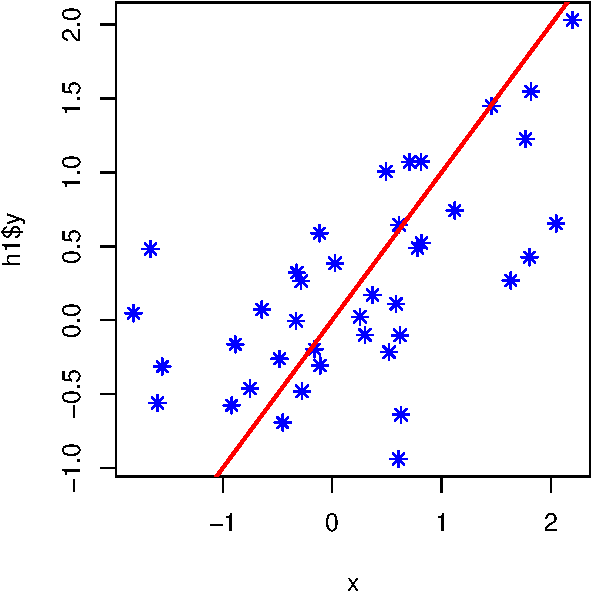
\includegraphics[keepaspectratio]{glspca_files/figure-pdf/h1plot-1.pdf}}

}

\caption{Type 1}

\end{figure}%

\begin{figure}[H]

{\centering \pandocbounded{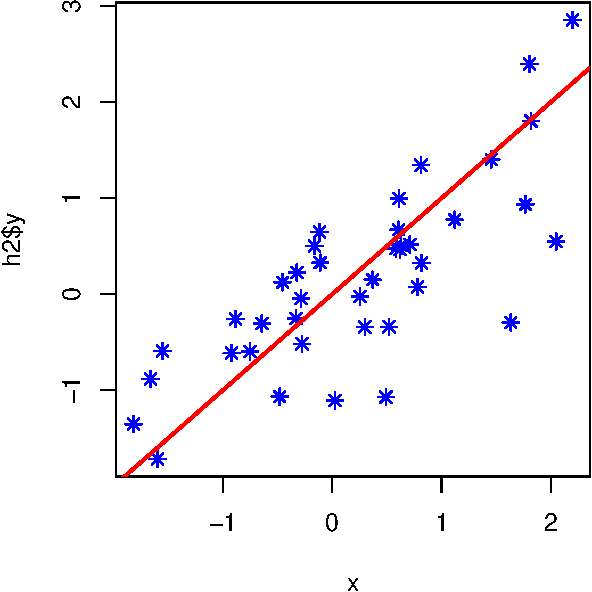
\includegraphics[keepaspectratio]{glspca_files/figure-pdf/h2plot-1.pdf}}

}

\caption{Type 2}

\end{figure}%

\begin{figure}[H]

{\centering \pandocbounded{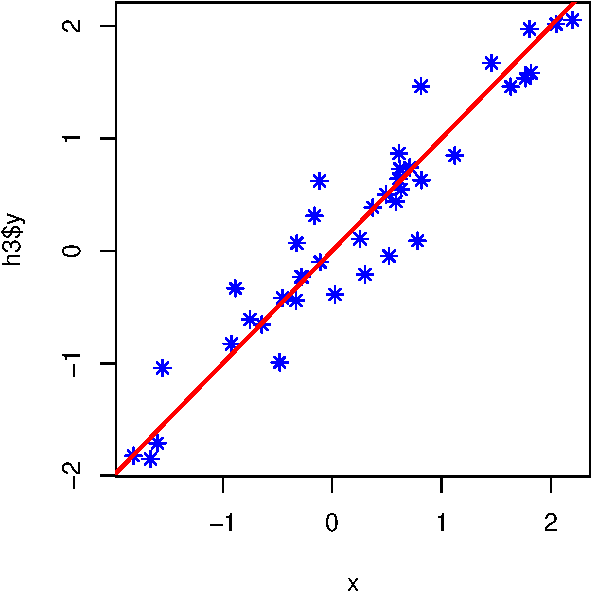
\includegraphics[keepaspectratio]{glspca_files/figure-pdf/h3plot-1.pdf}}

}

\caption{Type 3}

\end{figure}%

\section{Generalization}\label{generalization}

A far-reaching generalization of type 3 defines \(D=EMF'+AB'\), with
\(E\) and \(Q\) known matrices. In the unweighted case (and thus in the
update step of the majorization algorithm) this amounts to an SVD of the
residuals \(P_EXP_F\), where \(P_E\) and \(P_F\) are projectors on the
null spaces of \(E\) and \(F\).

\section{Correspondence Analysis}\label{correspondence-analysis}

\[
\sigma(A,B)=\text{tr}\ E^{-1}(F-AB')D^{-1}(F-AB')'
\] \# CCA

\[
\sigma(A,B)=\text{tr}\ (Z'EZ)^{-1}(Z'F-AB')D^{-1}(Z'F-AB')'
\] \# Canonical Analysis

\[
\sigma(A,B)=\text{tr}\ (X'X)^{-1}(X'Y-AB')(Y'Y)^{-1}(X'Y-AB')'
\]

\section{Redundancy Analysis}\label{redundancy-analysis}

\[
\sigma(A,B)=\text{tr}\ (X'X)^{-1}(X'Y-AB')(X'Y-AB')'
\]

\section{Aside}\label{aside}

\[
\sigma(A,B)=\mathbf{SSQ}(X-GAB'H')
\] with \(G\) and \(H\) known. \[
\sigma(A,B)=\text{tr}\ X'X-2\text{tr}\ X'GAB'H'+\text{tr}\ HBA'G'GAB'H'=\\
\text{tr}\ X'X-2\text{tr}\ H'X'GAB'+\text{tr}\ (H'H)BA'(G'G)AB'
\] Let \(\tilde B=(H'H)^\frac12 B\) and \(\tilde A=(G'G)^\frac12 A\).

Then \[
\text{tr}\ H'X'GAB'=\text{tr}\ (H'H)^{-\frac12}H'X'G(G'G)^{-\frac12}\tilde A\tilde B'
\] \[
\text{tr}\ (H'H)BA'(G'G)AB'=\text{tr}\ (H'H)(H'H)^{-\frac12}\tilde B\tilde A'(G'G)^{-\frac12}(G'G)(G'G)^{-\frac12}\tilde A\tilde B'(H'H)^{-\frac12}=\text{SSQ}(\tilde A\tilde B')
\]

Thus \[
\min_{A,B}\sigma(A,B)=\min_{A,B}\text{tr}(H'H)^{-1}(H'XG-AB')(G'G)^{-1}(H'XG-AB')'
\] which can be solved by an SVD of
\((H'H)^{-\frac12}H'X'G(G'G)^{-\frac12}\)

\section{Aside 2}\label{aside-2}

This generalizes type 3.

\[
\sigma(A,B,S)=\text{tr}\ U(X-GSH'-AB')V(X-GSH'-AB')'
\] Again it can be solved with a single SVD.

\subsection{Aside 3}\label{aside-3}

Suppose \(U\) and \(V\) are singular. Let

\[
U=\begin{bmatrix}K&K_\perp\end{bmatrix}
\begin{bmatrix}\Phi^2&0\\0&0\end{bmatrix}
\begin{bmatrix}K'\\K_\perp'\end{bmatrix}
\] \[
V=\begin{bmatrix}L&L_\perp\end{bmatrix}
\begin{bmatrix}\Psi^2&0\\0&0\end{bmatrix}
\begin{bmatrix}L'\\L_\perp'\end{bmatrix}
\] Let \(A=KP+K_\perp Q\) and \(B=LR+L_\perp S\).

\[
\text{SSQ}(U^\frac12(X-AB')V^\frac12)=
\text{SSQ}(\Phi K'XL\Psi-\Phi PR'\Psi)
\] which is minimizwed by the SVD of \(\Phi K'XL\Psi\).

\section{Elementwise weights}\label{elementwise-weights}

Use \(\text{vec}()\) \[
\sigma(Y)=\sum_{i=1}^n\sum_{j=1}^m w_{ij}(x_{ij}-y_{ij})^2
\] Now any \(V\geq W\) (elementwise) can be used to majorize.

\[
\sigma(Y)\leq\sigma(\tilde Y)-2\sum_{i=1}^n\sum_{j=1}^m w_{ij}(y_{ij}-\tilde y_{ij})(x_{ij}-\tilde y_{ij})+\sum_{i=1}^n\sum_{j=1}^m v_{ij}(y_{ij}-\tilde y_{ij})^2
\]

which leads to the majorization step of minimizing \[
\sum_{i=1}^n\sum_{j=1}^mv_{ij}(z_{ij}-y_{ij})^2
\] with \[
z_{ij}=\tilde y_{ij}+\frac{w_{ij}}{v_{ij}}(x_{ij}-\tilde y_{ij})
\] In Groenen, Giaquinto, and Kiers
(\citeproc{ref-groenen_giaquinto_kiers_03}{2003})
\(v_{ij}=\max_{j=1}^m w_{ij}\). In
(\citeproc{ref-deleeuw_}{\textbf{deleeuw\_?}})??
\(v_{ij}=\theta_i\xi_j\), where \(\theta\) and \(xi\) are chosen such
that \(\log\theta_i+\log\xi_j\geq\log w_{ij}\) and
\(\sum_{i=1}^n\sum_{j=1}^m(\log\theta_i+\log\xi_j)\) is minimized (a
linear programming problem)

\phantomsection\label{refs}
\begin{CSLReferences}{1}{0}
\bibitem[\citeproctext]{ref-groenen_giaquinto_kiers_03}
Groenen, P. J. F., P. Giaquinto, and H. A. L Kiers. 2003. {``{Weighted
Majorization Algorithms for Weighted Least Squares Decomposition
Models}.''} Econometric Institute Report EI 2003-09. Econometric
Institute, Erasmus University Rotterdam.
\url{https://repub.eur.nl/pub/1700}.

\end{CSLReferences}




\end{document}
